\graphicspath{{fig/lit_review/}}

\chapter{Literature review}
\label{cha:lit_review}

There exists a large body of literature relating to the phenomenon of collective
behaviour. Particularly unique to this literature is the variety of backgrounds
in which the authors are trained. Biologists, physicists, applied
mathematicians and statisticians have all made significant contributions to the
field of collective behaviour.

In this chapter we shall discuss some of the most important ideas and results
from the literature surrounding the study of collective behaviour. First, we
provide an overview and discussion of the evolutionary advantages which
collective behaviour affords individuals. After this we will discuss Eulerian
and Lagrangian models: the two main modelling paradigms used to simulate
flocking events. After this we shall review previous work which focused on
recording and utilising empirical data to assess predictive performance of
theoretical models.

\section{Biological function}
\label{sec:biological_function}

Behaving as a group can bring many advantages to the individuals involved. One
classically considered benefit of aggregation is an improved defence against
predation. Shoaling groups of fish have the ability to confuse predators, as
predators have difficulty selecting an individual target amongst a group
\parencite{landeau86}. In addition to this confusion effect, groups of
individuals can absorb and process more sensory information about their
environment than lone individuals are capable of, promoting the early detection
of predators \parencite{pitcher93}.

As well as providing defence against predation, behaving as a group can aid in
foraging for food as collections of individuals are able to gather more data
about their environment than solitary individuals \parencite{clark86}.
Collective motion is also understood to aid group navigation and migration,
with the suggestion that navigational accuracy increases with group size
through the ``many wrongs principle'' \parencite{simmons04}. For birds, group
navigation often brings an additional energetic advantage as individuals can
work to form aerodynamically efficient shapes \parencite{weimerskirch01}. As
well as these advantages, group living can aid in facilitating reproduction and
the rearing of young.

Despite the advantages afforded by collective behaviour, it isn't without its
dangers. For example, there is an understanding that flocking behaviours may
also have the unintended consequence of actually \emph{attracting} the
attention of predators \parencite{wittenberger85}. A more dramatic consequence
of collective behaviour can be seen in the formation of ant mills. Ant mills
occur when a group of foraging army ants become separated from the main column
of a raiding swarm \parencite{schneirla44}. Each ant follows the ant in front
of it, eventually causing the separated workers to run in a densely packed
circle until they all die from exhaustion \parencite{schneirla71}. This
phenomenon was first recorded in 1921, when William Beebe observed an ant mill
with a circumference of \SI{370}{\metre} \parencite{beebe21}. With a mill so
large, it took an individual ant 2.5 hours to make a single revolution of the
mill \parencite{surowiecki05}.

As we have seen, much of the \emph{why} of collective behaviour can be
understood by considering the evolutionary advantages which group behaviour
affords individuals of the group. However, we have still yet to broach the
\emph{how} of collective behaviour.

\section{Mathematical approaches}
\label{sec:models}

There has long been an appeal of using mathematics as a tool to understand
collective behaviour. These models of collective behaviour are broadly
partitioned into two paradigms: the Lagrangian and Eulerian approaches. These
descriptions are analogous to the models of fluid dynamics, where Lagrangian
models consider flow in terms of interactions of fluid parcels and Eulerian
models consider the changing fluid properties at a given point in space and
time. In the analogous models of collective behaviour, Lagrangian models
simulate the movements and interactions of individuals and Eulerian models
consider the changing properties of a group through space and time.

\subsection{Lagrangian models} \label{ssec:lagrangian_models}

So called agent-based models (ABMs), also referred to as Lagrangian models,
have proven a useful tool in modelling collective behaviours. In these models
the behaviour of an agent is simulated at the individual level. An agent's
behaviour is determined by social interactions with neighbouring individuals.
Examples of typical interactions include the desire to move in the same
direction as neighbours (alignment, or orientation), the desire to avoid
collisions (repulsion) and a desire to remain close to neighbours (attraction).
As well as simulating social behaviours, ABMs also specify how an individual
identifies neighbours with which to interact. An agent may, for example,
identify neighbours as those; within a certain distance (metric interaction);
positioned inside a field of vision or as one of a fixed number of closest
neighbours (topological interaction).

In a pioneering paper, \textcite{aoki82} developed an ABM to simulate the
movements of fish schooling in two-dimensions. Here it was shown that
collective behaviour can arise from simple interactions at an individual level,
\emph{without} the need of a leader, and \emph{without} each individual having
information about the movement of the group as a whole. The model simulated
zonal interactions in which the area around each fish was partitioned into
zones of repulsion, alignment and attraction (correspondingly: avoid, parallel
and approach in the original publication). The partitioning of space in this
way is illustrated in \cref{fig:zone_illustration}, and has remained a popular
idea in following literature. As well as zonal interactions this model
accounted for fish having incomplete fields of vision, that is: a blind spot
into which they cannot see. The simulation of a blind spot was utilised in
further studies. Later, other models were also devised to simulate fish schools
\parencite{okubo86, huth92}.

\begin{figure}[tb]
	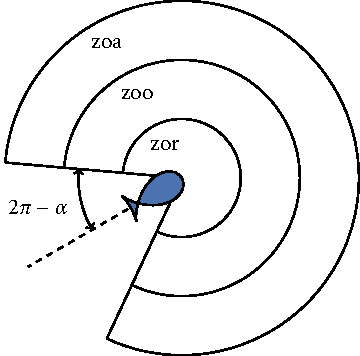
\includegraphics{zonal_tikz.pdf}
    \caption{An illustration of the area around an agent (here, a fish)
        partitioned into multiple zones, based on the work of
        \textcite{aoki82}. zor: zone of repulsion, zoo: zone of orientation (or
        alignment), zoa: zone of attraction. The missing segment behind the
        fish represents a blind zone into which it cannot see.}
	\label{fig:zone_illustration}
\end{figure}

Following this, \textcite{reynolds87} formulated a mathematical model,
motivated by the production of computer animations, which described the
movement of birds flocking in three-dimensional space. To produce more
aesthetically pleasing animations, the software, ``Boids'', implemented
additional sophistications such as banking during turns. This focus on
developing simulations which produce elegant behaviour made rigorous scientific
analysis difficult. Interestingly, Tim Burton's 1992 Batman Returns used a
modified version of the Boids software to simulate animations of bat swarms and
penguin flocks.

Substantially more complex than Boids was the software package Massive
(Multiple Agent Simulation System in Virtual Environment), originally developed
by Stephen Regelous for Peter Jackson's Lord of the Rings trilogy
\parencite{koeppel02}. This software was used to help generate the striking
battle sequences of the trilogy, where each individual orc, elf and other
miscellaneous creature of middle-earth was simulated according to the rules of
an agent based model \parencite{robbins17}. In 2004, Regelous received the
Scientific and Engineering Award from the Academy of Motion Picture Arts and
Sciences for his work on Massive. Since then, Massive has been used in films
such as Inception, Harry Potter and the order of the Phoenix, James Bond's
Spectre, and HBO's hit TV series Game of Thrones (\cref{fig:got}). With this
legacy in mind, in 2018 Regelous received an Emmy award to recognise his
contribution to the entertainment industry.

\begin{figure}[tb]
    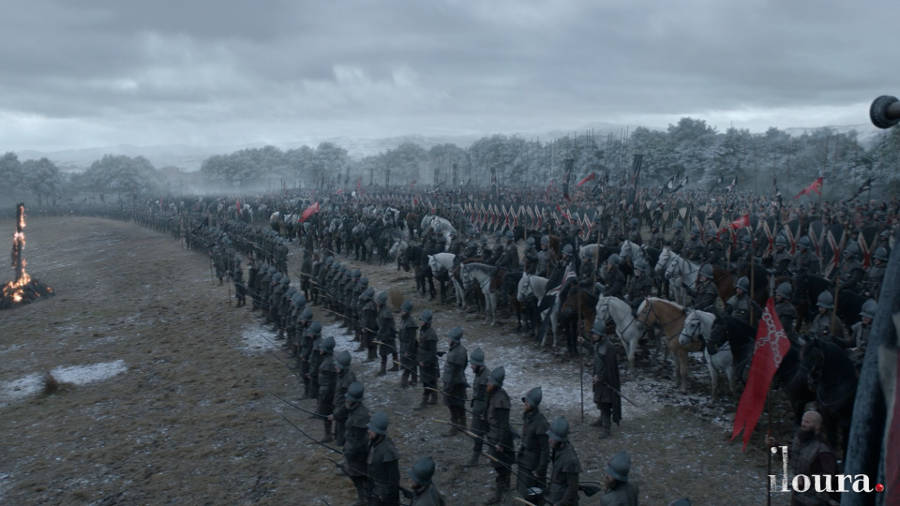
\includegraphics[width=\textwidth]{GOT.jpg}
    \caption{The animation company Iloura lent heavily on the Massive software
        to orchestrate army formations, fighting soldiers and horse actions for the
        dramatic scenes in HBO's Game of Thrones episode ``Battle of the Bastards''.}
    \label{fig:got}
\end{figure}

Not motivated by the lure of an Academy Award, but instead motivated by
research within statistical physics, \textcite{vicsek95} introduced a simple
two-dimensional model in which self-propelled particles move with a fixed
absolute velocity and align with neighbours within an interaction radius. This
model is commonly referred to as the ``Vicsek Model'' (VM). Despite its
simplicity this model produces complex behaviour resembling that of a real
biological system. \textcite{vicsek95} investigated the phase transition
between ordered and disordered motion as the density of particles and noise in
the system varied. This transition from order to disorder is an example of a
spontaneously breaking (rotational) symmetry, as the group has no preferred
direction of motion \emph{a priori}, but under simulation each group converges
upon some arbitrary direction to travel in. Because of this, the Vicsek model
stands as an apparent violation of the Mermin-Wagner Theorem, which states that
continuous symmetries cannot be spontaneously broken by systems that are able
to achieve long range order in dimensions $d\leq 2$ \parencite{mermin66}.
However, the Vicsek model is out of equilibrium and Mermin-Wagner only applies
to systems in equilibrium.

\begin{figure}[tb]
	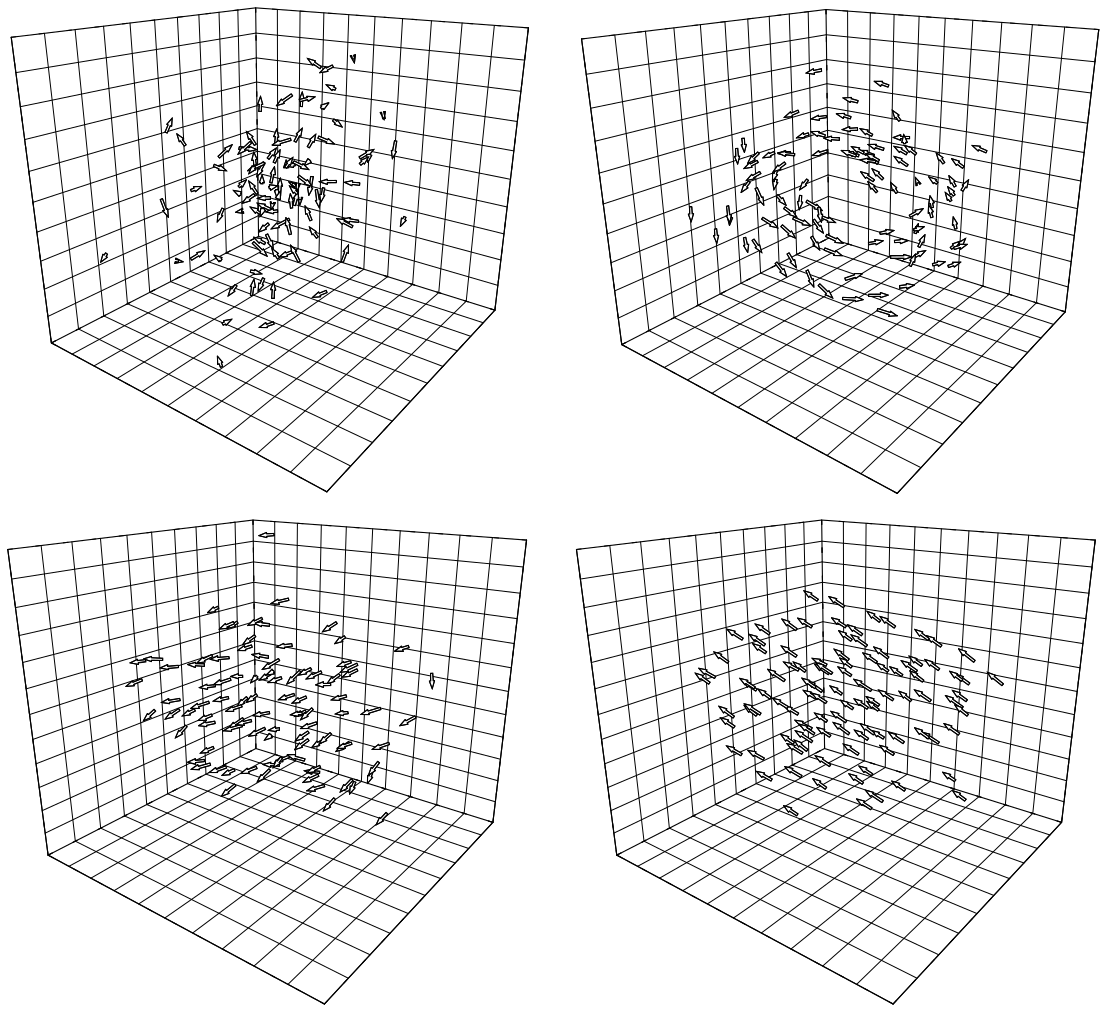
\includegraphics[width=0.75\textwidth]{couzin.png}
    \caption{Taken from \textcite{couzin02}, different steady-state
    solutions (swarm, torus, dynamically parallel and highly parallel) obtained
    by making small changes to model parameters of a three-dimensional flocking
    model.}
	\label{fig:couzin}
\end{figure}

Later, models were developed to explore the movements of mammals and other
vertebrate groups. Using a three-dimensional model that follows the zonal
approach of \textcite{aoki82}, \textcite{couzin02} showed major group-level
behavioural changes as minor changes in individual interaction rules were made.
With small changes in the model parameters, groups transitioned from
disordered, swarm-like behaviour, to toroidal milling structures, to forming
dynamic and highly parallel groups, as illustrated in \cref{fig:couzin}. In
addition to this the author's simulations demonstrated evidence of the
collective memory of a group, suggesting that previous group structure
influences future behaviour as interactions change.

Further research was made by \textcite{couzin05} which investigated how leaders
influence the motion of travelling groups. A zonal
repulsion-attraction-alignment model was used as the basis for this work. Here,
though, a proportion of the flock were given information about a preferred
direction of motion, and so balanced their social interactions with the desire
to move in this direction. Individuals in the flock did not know which members
of the group, if any, had information. Simulations showed that only a small
proportion of leaders are necessary to guide groups with a high degree of
accuracy. Further results investigated how groups of individuals make
collective decisions in the face of conflicting desires.

As a method for exploring collective behaviour, Lagrangian models are very
appealing in their intuitiveness and in the ease of implementing explicit
behavioural rules. Though for many years the simulation and exploration of
these models was limited by computing power; modern computation allows for the
simulations of large groups over many time steps. With these advances in
computing, and a growing interest in the field, a significant proportion of the
literature focuses on the analysis and exploration of agent-based models.

\subsection{Eulerian models} \label{ssec:eulerian_models}

Sometimes known as continuum models, Eulerian models are complementary to the
Lagrangian method and work at a coarse-grained level \parencite{giardina08}.
Eulerian models are typically constructed of a set of partial differential
equations which describe how density and other properties of a group develops
over time. This approach to modelling is often used to investigate the
long-time spatial and density properties of groups.

One such Eulerian approach by \textcite{gueron93} modelled the movements of
large groups of wildebeest. The predictions of the model were compared with
aerial observations of migrating wildebeest in the Serengeti
(\cref{fig:wildebeest}). The large-scale front patterns seen in the aerial
photography were reproduced by their model.

\begin{figure}[tb]
    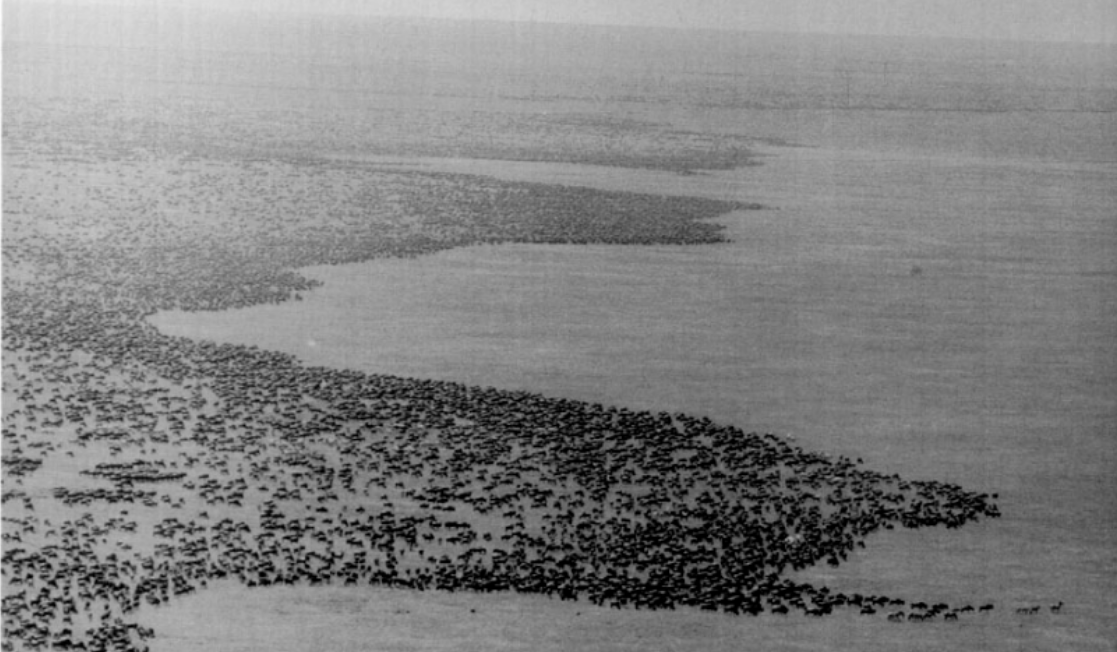
\includegraphics[width=\textwidth]{wildebeest.png}
    \caption{Aerial photography of migrating wildebeest showing large-scale
      front patterns, as presented in the work of \textcite{gueron93}.}
    \label{fig:wildebeest}
\end{figure}

Later, \textcite{toner98} introduced a quantitative continuum theory of
flocking. There are similarities between the hydrodynamic equations introduced
by the authors and the Navier-Stokes equation for simple incompressible fluids.
This model is capable of predicting the existence of an ordered phase of
motion, as is often observed in the field, and propagating density waves.
Detailed analysis of the model is made using techniques (e.g. dynamical
renormalization group) from nonequilibrium condensed matter physics and can be
used to make quantitative predictions of the properties of the long-distance,
long-time behaviour of the ordered state. Eulerian models have also been used
to analyse vortex solutions \parencite{topaz04} and stationary clump solutions
\parencite{topaz06}.

However, the Eulerian approach is limited. Most analyses are restricted to a
single dimension and the approach has not proven appropriate for modelling
groups of low densities \parencite{giardina08}. Additionally, these models
require more involved computer programming than their Lagrangian counterparts
necessitate. With this in mind, and with the advantages of the Lagrangian
approach, in this thesis we will concentrate entirely on modelling in the
Lagrangian framework.

\section{Empirical studies}
\label{sec:empirical_studies}

Models of collective motion rely on apriorstic assumptions about the properties
and behaviours of individuals. We also understand that the emergence of a
biologically realistic pattern from simulating a theoretical model \emph{is
not} sufficient evidence of model correctness. That is, the emergence of a
desired pattern is not evidence that a model is correctly capturing the
interactions of individuals. This observation is further compounded by the
understanding that models implementing different local interactions can produce
similar looking behaviour at the group level. As such, real data describing the
dynamics of animal aggregations is essential to assess the validity and
efficacy of theoretical models and the assumptions they make. With such data,
it would be possible to compare and rank the predictive performance of
competing models.

Thorough comparison between real data and model has proven difficult largely
because of the scarcity of appropriate data. The collection of suitable data
can be a complicated and convoluted process. Taking observations in the field
is technically demanding, requiring the precise calibration of sensitive
measurement equipment, not to mention the additional difficulty of the
typically three-dimensional nature of animal aggregations. Collecting data in a
laboratory setting seems an obvious workaround, however this imposes
restrictions on the types of behaviour which can be captured. A laboratory may
be an appropriate environment to capture the movements of fish in a tank, but
it certainly isn't appropriate to capture the movements of flocking birds.
Despite the difficulties associated with collecting data, significant effort
has been made to track the movements and dynamics of groups of individuals.

\begin{figure}[tb]
	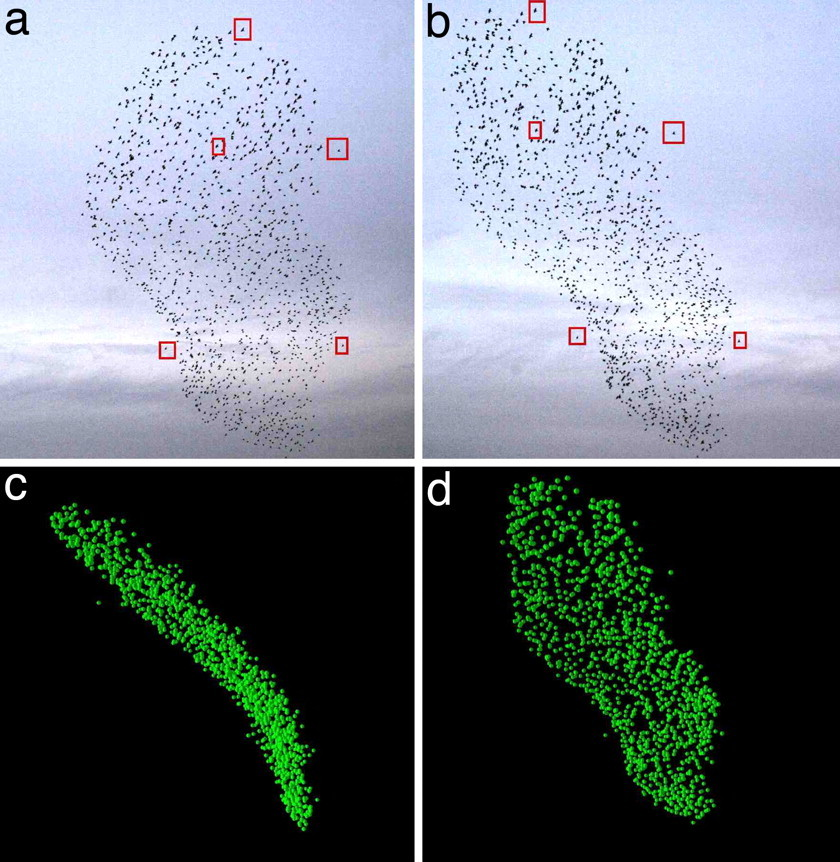
\includegraphics[width=0.75\textwidth]{ballerini_starlings.jpg}
    \caption{A flock of 1246 starlings reconstructed in three dimensions.
      Photographs taken at the same instant but $25$m apart (a--b) are used
      to reconstruct their three-dimensional positions (c--d). To perform
      reconstruction \textcite{ballerini08} needed to match each bird in (a)
      to its corresponding image in (b). The red squares show five matched
      pairs of birds.}
	\label{fig:ballerini}
\end{figure}

Initial work was limited to tracking small numbers of individuals in groups. In
these studies individuals were not linked through frames and hence the
collected data had no dynamic component. The first breakthrough came from
\textcite{cullen65} who used stereo photography to record the positions of fish
in three dimensions.

Fish are an appealing subject to study as experiments are easily conducted in a
laboratory setting. Furthermore, the movements of fish can effectively be
restricted to two dimensions by conducting the experiments in shallow water.
With these considerations, further research also concentrated on fish
\parencite{partridge80,van_long85}. Having collected empirical data, these
studies investigate properties such as the distance of individuals to their
nearest neighbour, or the direction from an individual toward their nearest
neighbour. Empirical studies were also made of small groups of flocking birds,
with similar statistics and properties realised \parencite{major78,budgey98}.

More recently, a breakthrough study by \textcite{ballerini08} reconstructed the
three-dimensional positions of flocks of starlings consisting of up to 2600
individual members (\cref{fig:ballerini}). To collect the data the authors
used a combination of stereometric and computer vision techniques. Having
collected and extracted the dataset, the authors began by constructing angular
density plots of nearest neighbours. These plots revealed a strong anisotropy
in the flock, with a lack of nearest neighbours positioned along the direction
of motion. Having investigated how this anisotropy decays as a function of
nearest neighbour, the authors concluded that interactions are not dependent on
metric distance (interactions with agents within a fixed distance), as most
models in the literature assume, but on a topological distance (interaction
with a fixed number of closest agents, irrespective of distance). This analysis
suggested that on average a starling interacts with between six and seven of
its closest neighbours.

\begin{figure}[tb]
	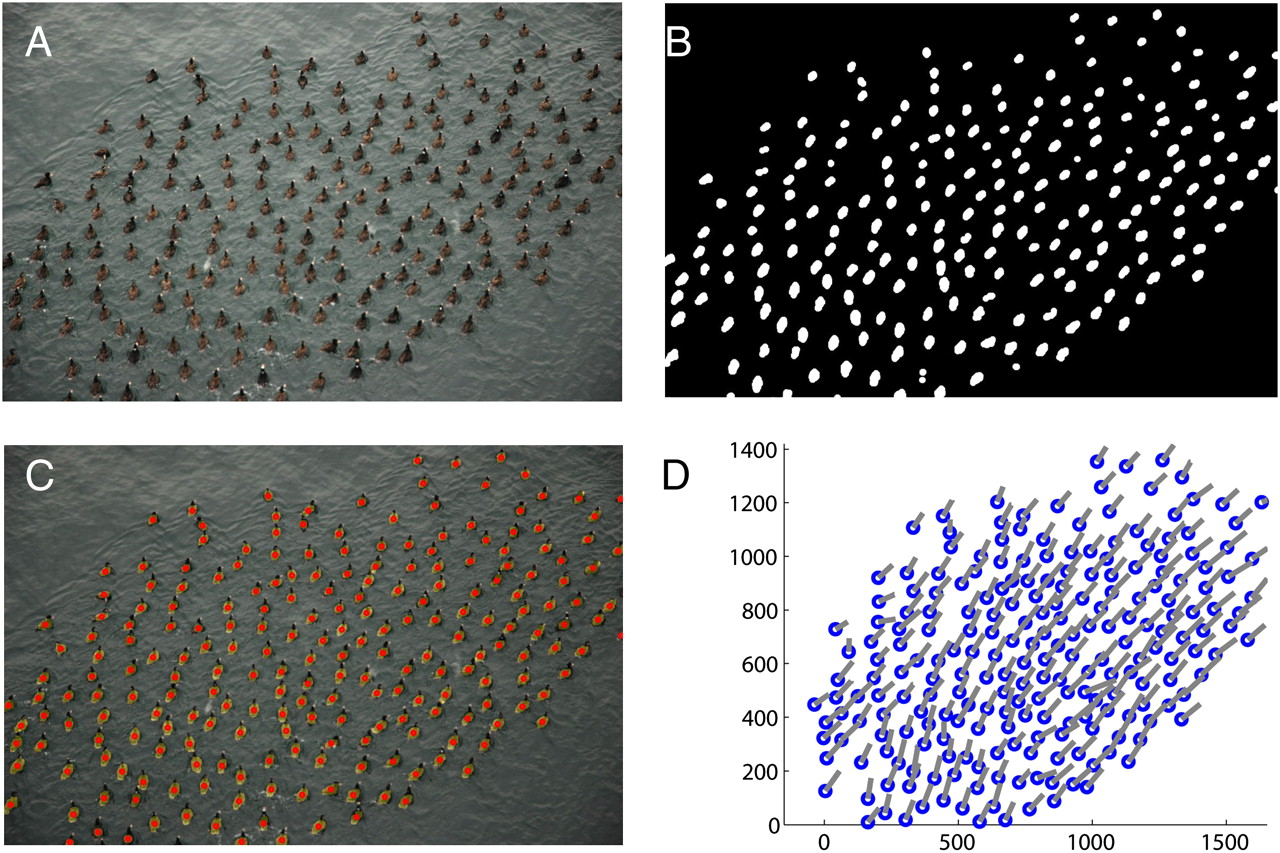
\includegraphics[width=\textwidth]{lukeman_data.jpg}
    \caption{An image of field data and visualisations of the transformations
        used to extract positions of individuals in a flock of foraging birds
        \parencite{lukeman10}.}
	\label{fig:lukeman_extraction}
\end{figure}

A significant contribution to the field was made by \textcite{lukeman10}, who
collected and analysed data of large numbers of diving ducks interacting on the
surface of a lake. Crucially, this dataset tracked individuals \emph{between}
frames and therefore allowed the reconstruction of a bird's trajectory through
space and time. This data showed an increase by a factor of ten the number of
individuals which could be reliably tracked though time \parencite{lukeman09}.
The extracted dataset was investigated and plots of nearest neighbour densities
were realised. It was observed from these plots that the highest density of
neighbours occurs at some preferred distance, in front of and behind the focal
bird. Further analysis fitted varying zonal models to the data. Optimal model
parameters were fitted to best reproduce the spatial neighbour densities and
density as a function of circumferential distance. It was concluded that a
zonal repulsion-alignment-attraction model with an additional frontal
interaction was best able to reproduce the desired spatial and angular
neighbour distributions.

Following this, \cite{katz11} investigated two and three fish shoals of golden
shiners. Data was recorded by placing fish in shallow tanks of water and using
custom tracking software to convert video footage into data describing the
centre of mass of individual fish through time. Working in a classical
mechanics framework the authors consider the effective forces acting on a focal
fish as a function of position and velocity. It was found that the dominant
interaction between fish was the regulation of their speed. No evidence was
found of explicit alignment of direction between individuals; instead,
alignment occurred as a product of attraction and repulsion between
individuals. Pairwise interactions were seen to predict the spatial
distributions of neighbours, and this observation was validated for shoals of
10 and 30 individuals.

Analysis of empirical data has so far focused on epiphenomena such as nearest
neighbour distances or angular neighbour densities. Research has then focused
on fitting models which are best able to replicate these properties, rather
than movements of individuals themselves. With technological and methodological
advances we expect that more and more empirical data will become available in
the future.

\section{Numerical studies}
\label{sec:numerical_studies}

\textcite{mann11} acknowledged that an important aspect of model fitting is
knowing the associated uncertainty of inferred parameters. The author discussed
the importance of quantifying uncertainty in parameter inference on collective
behaviour models, as the associated empirical datasets often have high levels
of noise. With the importance of capturing uncertainty in mind, Mann
demonstrated a fully Bayesian approach to parameter inference on data simulated
from a collective behaviour model. Here, in contrast to the more numerous
empirical studies, parameters were inferred on their ability to explain the
\emph{movements} of agents, as opposed to the ability to reproduce epiphenomena
such as nearest neighbour densities or angular neighbour distributions.

The agents in Mann's model moved under a weighted sum of alignment and
attraction. After ten time steps the simulated data transitioned from
disordered motion to a steady state rotating mill. The author then compared the
ability to infer the weighting parameter, interaction radius and other
properties of the agents in two situations: before and after the achievement of
a steady state. It was discovered that the interaction radius could not be
reliably inferred when the agents had formed the rotating mill structure,
although it could be inferred in the disordered motion before steady state.
This result can be understood by considering that stable groups present a
limited number of particle configurations, and are therefore less informative
than out of equilibrium groups.

Although not utilised frequently in the literature, such simulation studies
represent a useful aid in developing the statistical machinery to fit models of
collective behaviour to real data.

\section*{Conclusions}

Although our understanding of collective behaviour has developed considerably from
early speculations of telepathy, there still remain many unknowns. We saw
that the notion of biological fitness goes a long way to explaining the
\emph{why} of collective behaviour. However, we also reflected on how much is
unknown about the \emph{how} of collective behaviour.

Much of the literature was seen to have utilised mathematical models in an
attempt to understand the mechanics underlying the formation and maintenance of
flocks. Two popular modelling paradigms were introduced: the Eulerian, and the
Lagrangian. Considering the strengths and weaknesses of these approaches, we
concluded that the Lagrangian framework represents a more intuitive and
appealing paradigm to study collective behaviour.

Having considered a number of different Lagrangian models, we saw that many
different models were able to produce visually similar flocking events. We
argued that comparison between model and data was essential to assess the
predictive performance of these models. A review of the literature taking
measure of real-flocking events was detailed. Previous work has been limited by
the availability of data of real flocking events. When data of real events has
been utilised, the focus has been on fitting models to best reproduce
properties such as nearest-neighbour densities. We argue that the fitting
process should instead centre on explaining the \emph{movements} of the flock,
rather than some epiphenomena of the flock.

In this thesis we seek to address the short-comings of previous work. In
particular, we seek to fit theoretical models of collective behaviour to
observations of real events. In contrast with previous work, this fitting
process seeks to explain the \emph{movements} of the flock, rather than some
statistical properties of the flock. In addition to this, multiple competing
models will be fit to the same observations, allowing us to perform a
quantitative comparison of predictive performance.
